\documentclass[aspectratio=169,10pt]{beamer}

% --- Pacchetti di base ---
\usepackage{amsmath,amssymb}
\usepackage{booktabs}
\usepackage{tabularx}
\usepackage{adjustbox}
\usepackage{graphicx}
\usepackage{subcaption}
\usepackage{qrcode}
\usepackage{tikz}
\usetikzlibrary{arrows.meta,backgrounds,calc,positioning,shapes.multipart}
\usepackage[edges]{forest}

% --- Stile Forest per i Concrete Syntax Trees (Slide 4) ---
\forestset{
  cst tree/.style={
    for tree={
      l=0cm,
      l sep=0.20cm,
      inner sep=0.03cm,
      s sep=0.03cm,
      font=\fontsize{9.0}{10.5}\selectfont\ttfamily,
    }
  }
}

% --- Colori Personalizzati (Palette Bicocca & Deep Tech) ---
\definecolor{unimibBlue}{HTML}{0B3C68}
\definecolor{unimibRed}{HTML}{990000}
\definecolor{techAccent}{HTML}{1A5276}
\definecolor{cardBg}{HTML}{F8FAFC}
\definecolor{metricGreen}{HTML}{1E8449}
\colorlet{WHITE}{white}
\colorlet{BLACK}{black}

% --- Tema Cookie ---
\usetheme[
  accent=unimibBlue,
  progressbar=foot,
  sectionpage=progressbar,
  numbering=fraction,
  block=fill,
  fonts=none,
  mathfonts=none,
]{cookie}

% --- Regolazione Dimensioni Font Titoli e Struttura ---
\setbeamerfont{frametitle}{size=\fontsize{13}{16}\selectfont,series=\bfseries}
\setbeamerfont{number rail}{size=\fontsize{13}{16}\selectfont,series=\bfseries}
\setbeamerfont{cookie kicker}{size=\fontsize{7.5}{9.5}\selectfont,series=\bfseries}

% --- Margini compatti per sfruttare al meglio lo spazio orizzontale ---
\setbeamersize{text margin left=0.045\paperwidth, text margin right=0.040\paperwidth}

% --- Rientro compatto per elenchi puntati e numerati (elimina il margine bianco eccessivo) ---
\setlength{\leftmargini}{1.15em}
\setlength{\leftmarginii}{1.15em}
\setlength{\leftmarginiii}{1.15em}
\setbeamertemplate{itemize/enumerate body begin}{\setlength{\leftmargini}{1.15em}}
\setbeamertemplate{itemize/enumerate subbody begin}{\setlength{\leftmarginii}{1.15em}}
\setbeamertemplate{itemize item}{\raisebox{0.12ex}{\scriptsize\color{unimibBlue}$\blacktriangleright$}}
\setbeamertemplate{itemize subitem}{\raisebox{0.12ex}{\tiny\color{techAccent}$\blacktriangleright$}}

% --- Metadati Presentazione ---
\title[OmniDeps]{A Language-Agnostic Framework\\ for Dependency Extraction}
\subtitle{Master's Thesis in Computer Science}
\author[C. Ferrario]{Christian Ferrario}
\institute{University of Milano-Bicocca}
\date{A.Y. 2025--2026}

% ==============================================================================
% TEMPLATE PERSONALIZZATO PER IL FRONTESPIZIO (Slide 1)
% Proporzionato, elegante, senza collisioni con il cuneo grafico
% ==============================================================================
\setbeamertemplate{title page}{%
  \begin{tikzpicture}[remember picture,overlay]
    % Cuneo diagonale Bicocca Blue
    \coordinate (cuttop) at ($(current page.north east)+(-0.34\paperwidth,0)$);
    \coordinate (cutbottom) at ($(current page.south east)+(-0.46\paperwidth,0)$);
    \fill[unimibBlue] (cuttop) -- (current page.north east) -- (current page.south east) -- (cutbottom) -- cycle;
    % Badge elegante con Logo Bicocca nel cuneo
    \node[anchor=center,fill=white,rounded corners=4pt,inner sep=8pt,draw=cookieLine!30,line width=0.5pt]
      at ($(current page.east)+(-0.18\paperwidth,0)$) {
        
\includegraphics[width=0.22\paperwidth,keepaspectratio]{../images/logo_unimib.pdf}
      };
  \end{tikzpicture}%
  % Colonna testuale sinistra (larghezza 0.52\paperwidth, isolata dal cuneo)
  \vspace*{0.02\paperheight}%
  \begin{minipage}[t]{0.52\paperwidth}
    \raggedright
    \cookiekicker{UNIVERSITÀ DEGLI STUDI DI MILANO-BICOCCA}\par\vspace{0.15em}
    {\fontsize{7.5}{9.5}\selectfont\color{cookieMuted}Dipartimento di Informatica, Sistemistica e Comunicazione\par}
    \vspace{0.9em}
    {\fontsize{16.5}{20}\selectfont\bfseries\color{unimibBlue} A Language-Agnostic\\[0.06em]Framework for Dependency\\[0.06em]Extraction\par}
    \vspace{0.45em}
    {\fontsize{8.5}{10.5}\selectfont\color{cookieMuted}Master's Thesis in Computer Science\par}
    \vspace{0.65em}
    {\color{unimibBlue}\rule{0.14\paperwidth}{1.3pt}}\par
    \vspace{0.85em}
    {\scriptsize\textbf{Candidate:}}\par\vspace{0.1em}
    {\small\bfseries Christian Ferrario\par}
    \vspace{0.65em}
    {\scriptsize\textbf{Supervisor:} Prof. Francesca Arcelli Fontana\par}
    \vspace{0.15em}
    {\scriptsize\textbf{Co-Supervisor:} Dr. Francesco Refolli\par}
    \vspace{0.75em}
    {\scriptsize\color{cookieMuted}Academic Year 2025--2026}
  \end{minipage}%
}

\begin{document}

% ==============================================================================
% SLIDE 1: FRONTESPIZIO
% ==============================================================================
\begin{frame}[plain,noframenumbering]
  \titlepage
\end{frame}

% ==============================================================================
% SLIDE 2: CONTESTO & MOTIVAZIONE
% ==============================================================================
\begin{frame}{Context: Software Evolution \& Dependency Analysis}
  \cookiekicker{CONTEXT \& MOTIVATION}\par\vspace{0.4em}
  
  \begin{itemize}\setlength{\itemsep}{0.65em}
    \item \textbf{Software Evolution \& Technical Debt:}\\
      {\small Continuous evolution leads to architectural degradation, threatening long-term maintainability.}
      
    \item \textbf{Why Static Dependency Graphs?}
      \begin{itemize}\setlength{\itemsep}{0.25em}
        \item \textbf{Detect Architectural Smells:} {\small Uncover cyclic dependencies, unstable coupling, and modular decay.}
        \item \textbf{Impact Analysis \& Refactoring:} {\small Trace ripple effects before altering critical components.}
        \item \textbf{System Comprehension:} {\small Provide an accurate structural map of large codebases.}
      \end{itemize}
      
    \item \textbf{The Polyglot Challenge:}\\
      {\small Enterprise systems routinely combine multiple languages (Java, Python, C/C++, Rust).}
  \end{itemize}

\end{frame}

% ==============================================================================
% SLIDE 3: STATO DELL'ARTE & FRAMMENTAZIONE
% ==============================================================================
\begin{frame}{State of the Art: Tooling Fragmentation}
  \cookiekicker{LIMITATIONS OF EXISTING TOOLS}\par\vspace{0.4em}
  
  \begin{columns}[c,onlytextwidth]
    \column{0.48\textwidth}
      \begin{itemize}\setlength{\itemsep}{0.65em}
        \item \textbf{Coupling to Language Ecosystems:}\\
          {\small Tools are tied to specific compiler front-ends and native tooling (\texttt{javac}, Clang).}
          
        \item \textbf{Re-engineering Analysis Pipelines:}\\
          {\small Parsing, scoping, and graph generation must be rebuilt from scratch for every language.}
          
        \item \textbf{Heavyweight Multi-Language Tooling:}\\
          {\small Supporting multiple languages forces tools to bundle and maintain all underlying dependencies.}
          
        \item \textbf{Duplicated Engineering \& Fragmentation:}\\
          {\small Results in inefficient development, redundant effort, and fragmented tools.}
      \end{itemize}

    \column{0.48\textwidth}
      \centering
      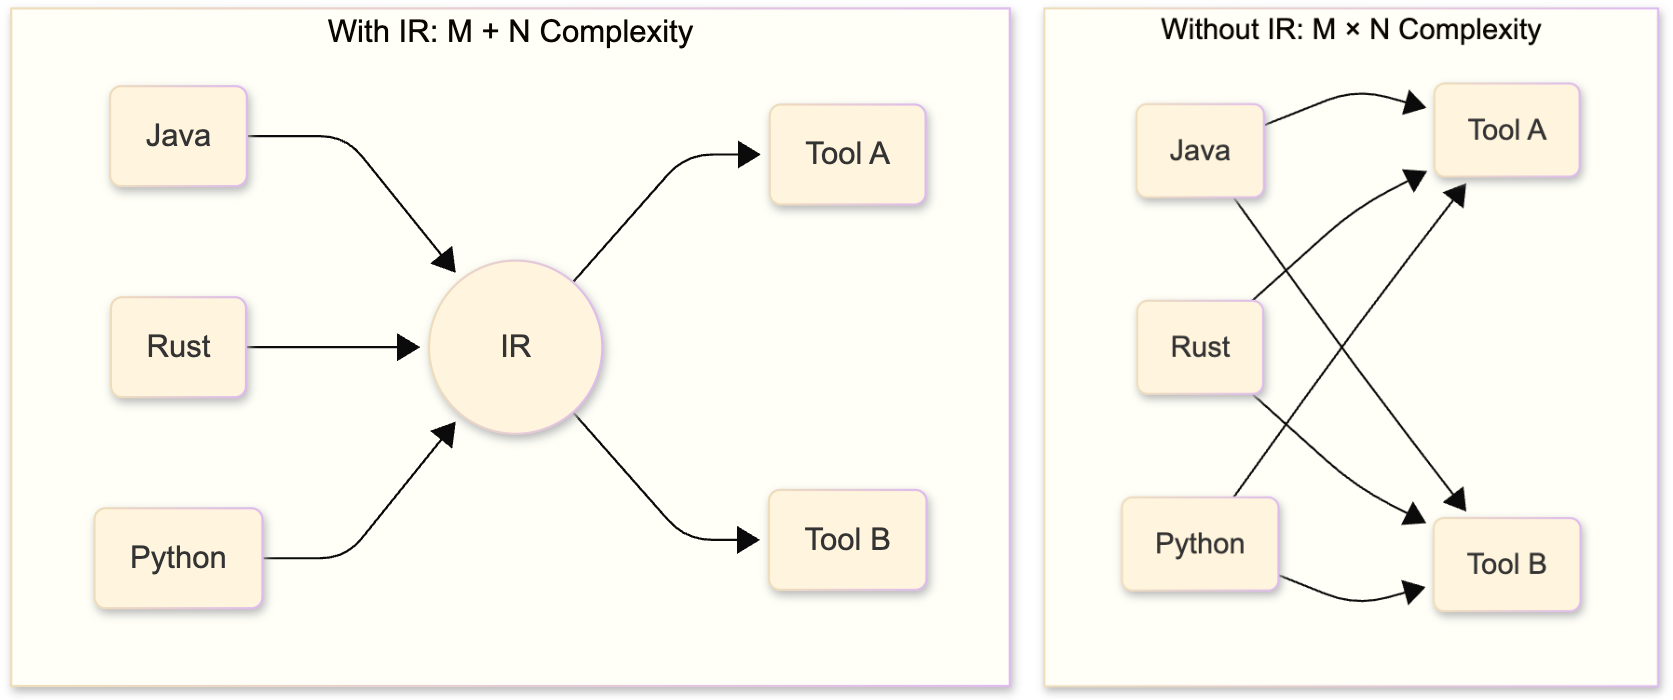
\includegraphics[width=\linewidth,height=0.52\textheight,keepaspectratio]{../images/background/mxn_problem.png}
      \vspace{0.2em}
      \captionof{figure}{\scriptsize Tool proliferation ($M \times N$) vs unified IR ($M + N$).}
  \end{columns}

\end{frame}

% ==============================================================================
% SLIDE 4: L'INTUIZIONE DEI CST
% ==============================================================================
\begin{frame}{Key Insight: Structural Convergence of CSTs}
  \cookiekicker{FOUNDATIONAL INSIGHT}\par\vspace{0.4em}
  
  \begin{columns}[c,onlytextwidth]
    \column{0.40\textwidth}
      \textbf{Generic Parsers (Tree-sitter):}\\
      {\small Generates Concrete Syntax Trees (CSTs) from formal grammars across 40+ languages.}
      
      \vspace{0.5em}
      \textbf{Structural Convergence:}\\
      {\small Despite lexical differences, equivalent architectural patterns yield structurally aligned syntax trees.}
          
      \vspace{0.5em}
      \textbf{Foundational Assumption:}\\
      {\small Code already compiles and is valid; extraction targets dependency topology without duplicating compiler checks.}

    \column{0.58\textwidth}
      \centering
      {\scriptsize\textbf{CST Comparison for} \texttt{a.b.c().d.e()}}\par\vspace{0.25em}
      \begin{minipage}[t]{0.485\linewidth}
        \centering
        {\scriptsize\textbf{(a) Rust CST}}\\[0.15em]
        \begin{adjustbox}{max width=\linewidth,max totalheight=0.62\textheight}
          \begin{forest}
            cst tree
            [call\_expression
              [field\_expression
                [field\_expression
                  [call\_expression
                    [field\_expression
                      [field\_expression
                        [identifier]
                        [field\_identifier]
                      ]
                      [field\_identifier]
                    ]
                    [argument]
                  ]
                  [field\_identifier]
                ]
                [field\_identifier]
              ]
              [argument]
            ]
          \end{forest}
        \end{adjustbox}
      \end{minipage}\hspace{0.015\linewidth}%
      \begin{minipage}[t]{0.485\linewidth}
        \centering
        {\scriptsize\textbf{(b) Python CST}}\\[0.15em]
        \begin{adjustbox}{max width=\linewidth,max totalheight=0.62\textheight}
          \begin{forest}
            cst tree
            [call
              [attribute
                [attribute
                  [call
                    [attribute
                      [attribute
                        [identifier]
                        [identifier]
                      ]
                      [identifier]
                    ]
                    [argument\_list]
                  ]
                  [identifier]
                ]
                [identifier]
              ]
              [argument\_list]
            ]
          \end{forest}
        \end{adjustbox}
      \end{minipage}
      \vspace{0.25em}
      \captionof{figure}{\scriptsize Structural convergence across languages for identical call semantics.}
  \end{columns}

\end{frame}

% ==============================================================================
% SLIDE 5: OBIETTIVI E OMNIDEPS
% ==============================================================================
\begin{frame}{Research Objectives \& OmniDeps Proposal}
  \cookiekicker{FRAMEWORK OVERVIEW}\par\vspace{0.3em}
  
  {\small Design, formalize, and implement \textbf{OmniDeps}: an extensible, language-agnostic static analysis framework for extracting architectural dependency graphs.}\par\vspace{0.3em}

  \begin{columns}[T,onlytextwidth]
    \column{0.32\textwidth}
      \begin{cookiecard}[title={Formal IR},height=3.8cm]
        \fontsize{7.5}{9.5}\selectfont
        \textbf{Universal Data Model:}\\
        Algebraic Data Types abstracting away syntactic peculiarities.\par\vspace{0.35em}
        \textbf{Structural Normalization:}\\
        Standardizes modules, composite types, and invocations into uniform IR entities.
      \end{cookiecard}

    \column{0.32\textwidth}
      \begin{cookiecard}[title={Rust Engine},height=3.8cm]
        \fontsize{7.5}{9.5}\selectfont
        \textbf{Functional Pipeline:}\\
        Decoupled 3-phase design ($\epsilon \to \rho \to \gamma$) ensuring type safety and memory robustness.\par\vspace{0.35em}
        \textbf{Query Algebra:}\\
        Symbol resolution via scope tree climbing without compiler coupling.
      \end{cookiecard}

    \column{0.32\textwidth}
      \begin{cookiecard}[title={Empirical Benchmark},height=3.8cm]
        \fontsize{7.5}{9.5}\selectfont
        \textbf{Graph Harmonization:}\\
        Semantic alignment methodology for fair cross-tool comparisons.\par\vspace{0.35em}
        \textbf{Large-Scale Evaluation:}\\
        Evaluated on 156 open-source projects ($\sim$98M LOC) against Arcan, Depends, and Entangle.
      \end{cookiecard}
  \end{columns}

  \vspace{0.3em}
  {\fontsize{7.0}{8.5}\selectfont\color{cookieMuted}%
    \textbf{Target Evaluation Languages:} Java, C, C++, Python, and Rust were selected to validate the methodology across diverse programming paradigms (OOP, systems, scripting), demonstrating the language-agnostic extensibility of the architecture.%
  }
\end{frame}

% ==============================================================================
% SLIDE 6: ARCHITETTURA DELLA PIPELINE
% ==============================================================================
\begin{frame}{Analysis Pipeline Overview}
  \cookiekicker{FUNCTIONAL COMPOSITION \& TYPE SAFETY}\par\vspace{0.2em}

  {\small
  $$\phi : \mathcal{W} \to \mathcal{G}, \qquad \phi = \gamma \circ \rho \circ \varepsilon = \gamma \circ (\rho_{\text{exec}} \circ \rho_{\text{build}}) \circ \varepsilon$$
  }\par\vspace{0.1em}

  \begin{columns}[T,onlytextwidth]
    \column{0.32\textwidth}
      \textbf{Phase 1: Extraction ($\varepsilon$)}\par\vspace{0.15em}
      {\fontsize{7.5}{9.2}\selectfont
      $\varepsilon : \mathcal{W} \to \mathcal{D}$\par
      Parses raw CSTs via Tree-sitter and applies heuristic pruning into unlinked IR. Only phase aware of native syntax.
      }

    \column{0.34\textwidth}
      \textbf{Phase 2: Resolution ($\rho$)}\par\vspace{0.15em}
      {\fontsize{7.5}{9.2}\selectfont
      $\rho : \mathcal{D} \to \mathcal{D}_{\text{res}}$\par
      Builds Scope Tree ($\rho_{\text{build}}$) and resolves symbolic identifiers ($\rho_{\text{exec}}$) via algebraic scope climbing. Purely logical.
      }

    \column{0.31\textwidth}
      \textbf{Phase 3: Graph ($\gamma$)}\par\vspace{0.15em}
      {\fontsize{7.5}{9.2}\selectfont
      $\gamma : \mathcal{D}_{\text{res}} \to \mathcal{G}$\par
      Flattens resolved entities into component vertices ($V$) and emits directed dependency edges ($E$). Purely structural.
      }
  \end{columns}

  \vspace{0.35em}
  \centering
  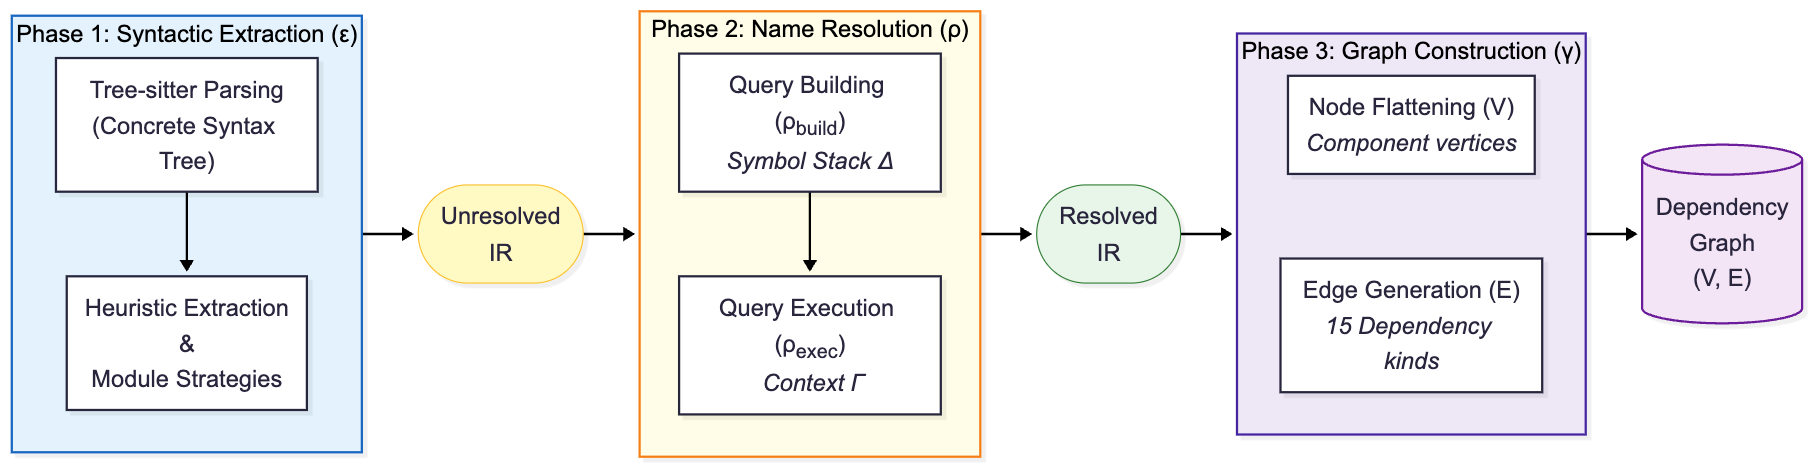
\includegraphics[width=0.96\textwidth,height=0.38\textheight,keepaspectratio]{../images/analysis_process/pipeline_detailed.png}
\end{frame}

% ==============================================================================
% SLIDE 7: FASE 1 - EXTRACTION & PRUNING
% ==============================================================================
\begin{frame}{Fase 1: Estrazione Sintattica e CST Pruning}
  \cookiekicker{DALLA SINTASSI ALL'IR}
  \vspace{0.1em}
  \begin{columns}[c,onlytextwidth]
    \column{0.48\textwidth}
      \begin{cookiecard}[title={Filtraggio Euristico del Rumore}]
        \small
        \begin{itemize}\setlength{\itemsep}{0.2em}
          \item \textbf{CST Pruning:} Rimozione dei token accessori (punteggiatura, keyword) tramite pattern matching.
          \item \textbf{Modular Boundaries:} Estrazione di namespace, package e file.
          \item \textbf{Structured Types:} Classi, struct, interfacce, trait ed enum.
          \item \textbf{Behavioral Elements:} Funzioni, metodi, invocazioni e istanziazioni.
        \end{itemize}
      \end{cookiecard}

    \column{0.50\textwidth}
      \centering
      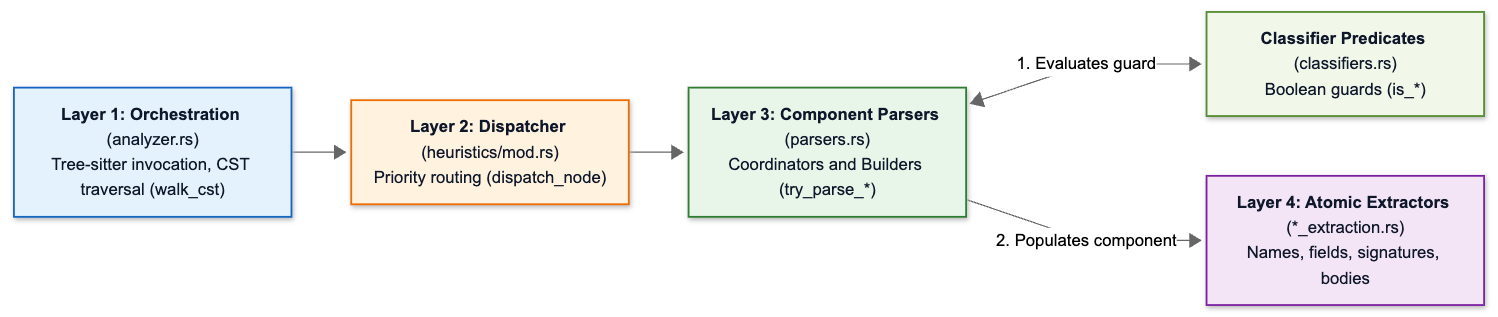
\includegraphics[width=\linewidth,height=0.52\textheight,keepaspectratio]{../images/extraction/extraction_layers.png}
      \vspace{0.2em}
      \captionof{figure}{\scriptsize Stratificazione dal CST nativo all'IR universale.}
  \end{columns}

\end{frame}

% ==============================================================================
% SLIDE 8: FORMALIZZAZIONE IR & TYPEREF
% ==============================================================================
\begin{frame}{Formalizzazione IR e Ciclo di Vita di TypeRef}
  \cookiekicker{MODELLAZIONE DEI TIPI ALGEBRICI}
  \vspace{0.1em}
  \begin{columns}[c,onlytextwidth]
    \column{0.48\textwidth}
      \begin{cookiecard}[title={Macchina a Stati del TypeRef}]
        \footnotesize
        \begin{itemize}\setlength{\itemsep}{0.2em}
          \item $\mathbf{Unresolved}(\pi_{\text{raw}})$: Riferimento sintattico grezzo.
          \item $\mathbf{ResolvedInternal}(\pi_{\text{res}}, \tau_{\text{path}})$: Entità interna al progetto.
          \item $\mathbf{ResolvedExternal}(\pi_{\text{res}})$: Dipendenza da libreria esterna.
          \item $\mathbf{Primitive}$ / $\mathbf{Failed}$: Tipi built-in o non risolti.
          \item \textbf{Coppia Oggetto-Membro $\langle \tau_{\text{path}}, \tau_{\text{type}} \rangle$:} In \texttt{c.addr}, traccia sia il tipo proprietario sia il membro.
        \end{itemize}
      \end{cookiecard}

    \column{0.50\textwidth}
      \centering
      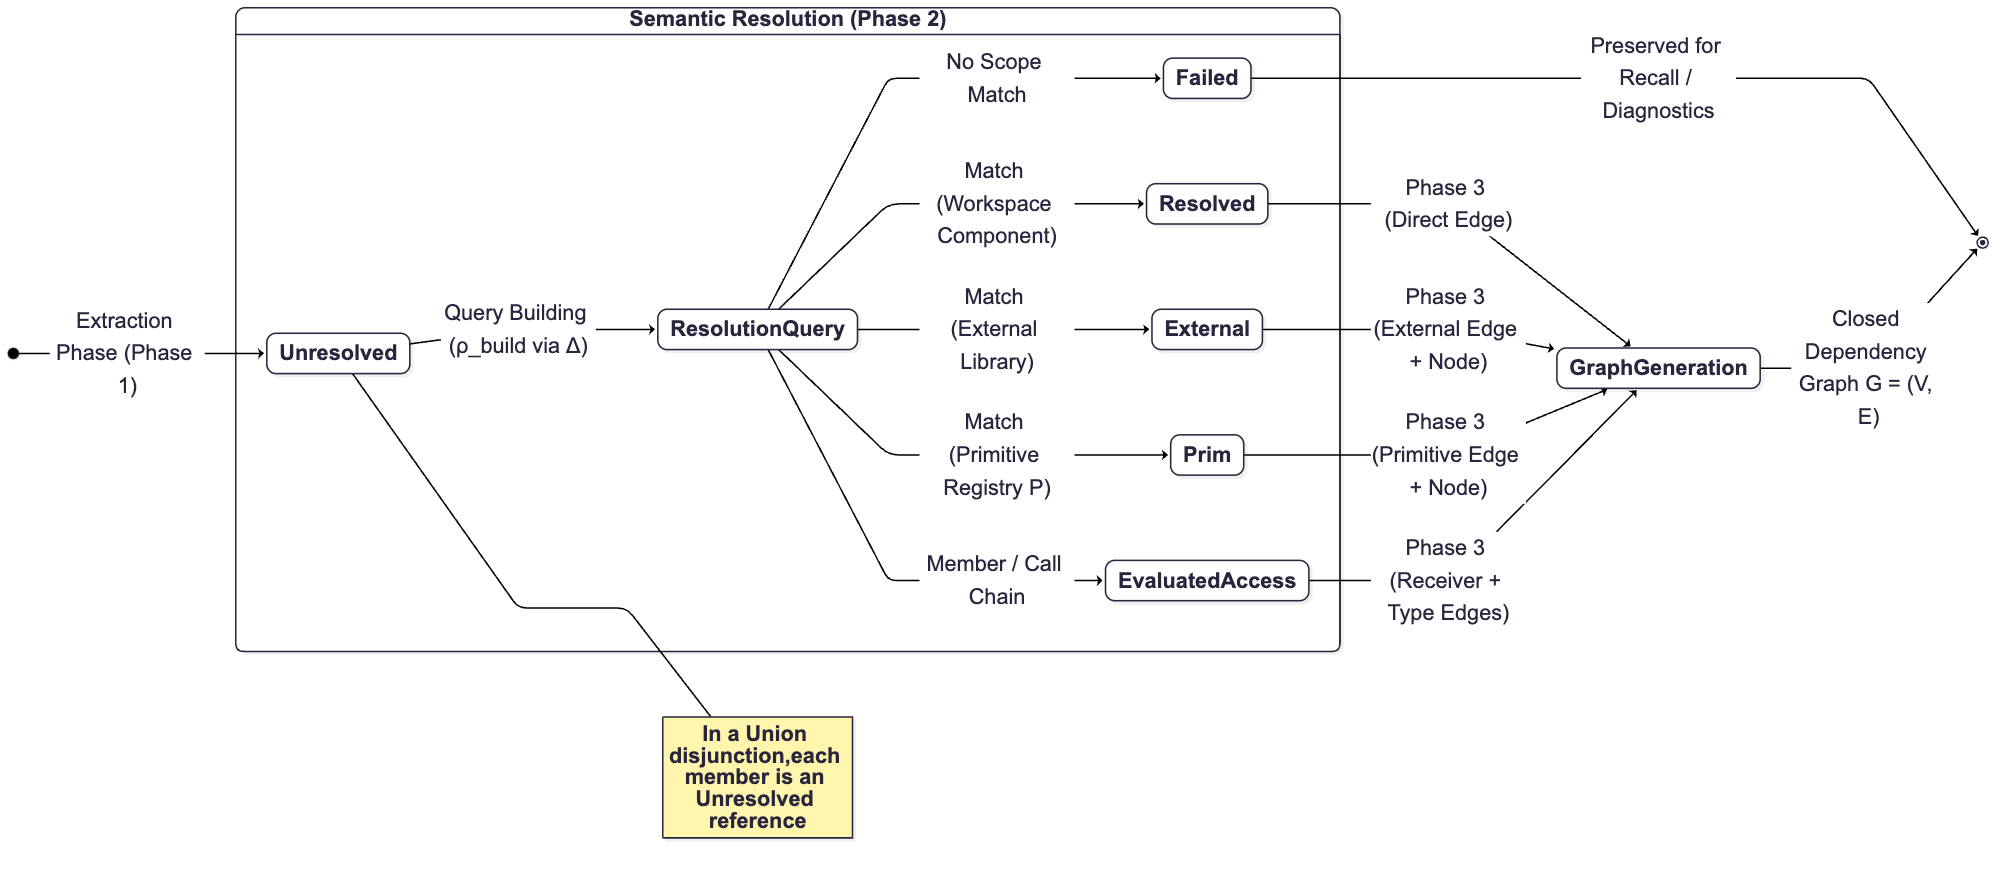
\includegraphics[width=\linewidth,height=0.52\textheight,keepaspectratio]{../images/formal_ir/typeref_lifecycle.png}
      \vspace{0.2em}
      \captionof{figure}{\scriptsize Ciclo di vita del tipo TypeRef dall'estrazione alla risoluzione.}
  \end{columns}

\end{frame}

% ==============================================================================
% SLIDE 9: FASE 2 - RISOLUZIONE DEI NOMI DISACCOPPIATA
% ==============================================================================
\begin{frame}{Fase 2: Risoluzione dei Nomi Disaccoppiata}
  \cookiekicker{NAME RESOLUTION ARCHITECTURE}
  \vspace{0.1em}
  \begin{columns}[c,onlytextwidth]
    \column{0.48\textwidth}
      \begin{cookiecard}[title={Disaccoppiamento in Due Passi}]
        \small
        \begin{enumerate}\setlength{\itemsep}{0.25em}
          \item \textbf{Query Building ($\rho_{\text{build}}$):} Uno \textit{Symbol Stack} locale ed effimero elimina variabili e parametri, traducendo i riferimenti in formule algebriche chiuse ($q \in \mathcal{Q}$).
          \item \textbf{Query Execution ($\rho_{\text{exec}}$):} Valutazione deterministica globale sullo Scope Tree del workspace, senza stato locale né dipendenza dall'ordine dei file.
        \end{enumerate}
      \end{cookiecard}

    \column{0.50\textwidth}
      \centering
      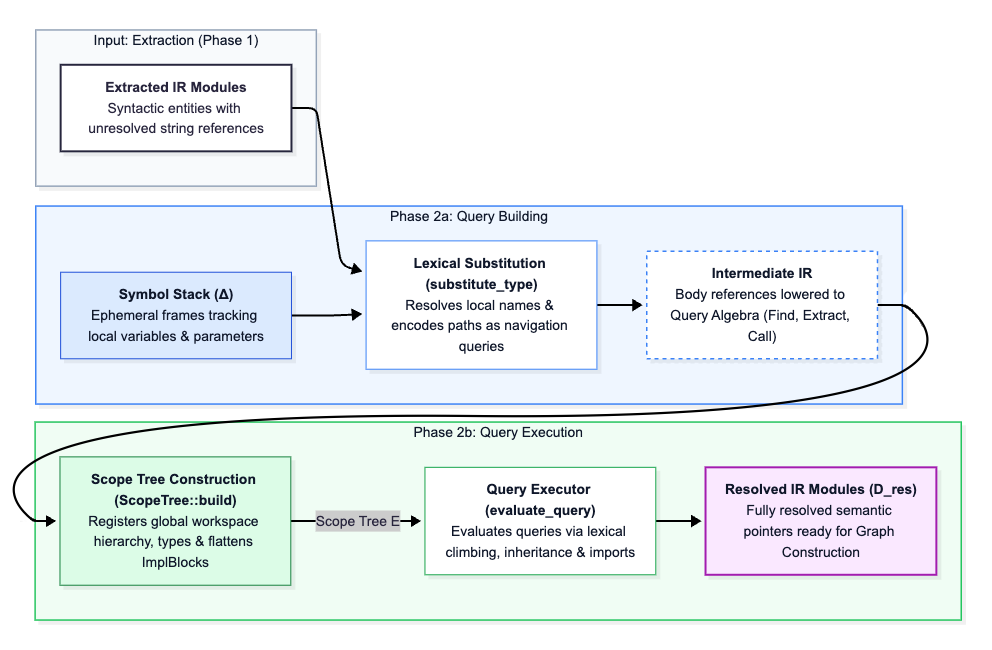
\includegraphics[width=\linewidth,height=0.52\textheight,keepaspectratio]{../images/name_resolution/two_phase_resolution.png}
      \vspace{0.2em}
      \captionof{figure}{\scriptsize Architettura di risoluzione disaccoppiata in due passi.}
  \end{columns}

\end{frame}

% ==============================================================================
% SLIDE 10: L'ALGEBRA DELLE QUERY
% ==============================================================================
\begin{frame}{L'Algebra delle Query: Tre Primitive}
  \cookiekicker{QUERY ALGEBRA}\par\vspace{0.1em}
  Tre sole primitive algebriche sono sufficienti a esprimere e risolvere qualsiasi riferimento:
  \vspace{0.15em}

  \begin{columns}[T,onlytextwidth]
    \column{0.32\textwidth}
      \begin{cookiecard}[title={Primitiva Find}]
        \small \textbf{Risalita Lessicale}
        \begin{itemize}\setlength{\itemsep}{0.1em}
          \item Risale lo Scope Tree finché il simbolo $\iota$ viene trovato.
        \end{itemize}
      \end{cookiecard}

    \column{0.32\textwidth}
      \begin{cookiecard}[title={Primitiva Extract}]
        \small \textbf{Discesa Strutturale}
        \begin{itemize}\setlength{\itemsep}{0.1em}
          \item Cerca il membro $\iota$ nel tipo risultante da $q$.
        \end{itemize}
      \end{cookiecard}

    \column{0.32\textwidth}
      \begin{cookiecard}[title={Primitiva Call}]
        \small \textbf{Propagazione Ritorno}
        \begin{itemize}\setlength{\itemsep}{0.1em}
          \item Valuta il callable $q$ e propaga il tipo di ritorno.
        \end{itemize}
      \end{cookiecard}
  \end{columns}
  \vspace{0.2em}

  \begin{cookiecard}[title={Composizione Algebrica per Invocazioni Concatenate}]
    \centering\footnotesize
    $\mathbf{Extract}\Big(\mathbf{Call}\Big(\mathbf{Extract}\Big(\mathbf{Call}\Big(\mathbf{Extract}(\mathbf{Find}(order), \text{getCustomer})\Big), \text{getAddress}\Big)\Big)$
  \end{cookiecard}

\end{frame}

% ==============================================================================
% SLIDE 11: VALUTAZIONE TOPOLOGICA & ARENA RUST
% ==============================================================================
\begin{frame}{Valutazione Topologica: Scope Tree Arena}
  \cookiekicker{INGEGNERIA E PRESTAZIONI IN RUST}
  \vspace{0.1em}
  \begin{columns}[c,onlytextwidth]
    \column{0.48\textwidth}
      \begin{cookiecard}[title={Arena Allocation in Rust}]
        \small
        \begin{itemize}\setlength{\itemsep}{0.2em}
          \item \textbf{Allocazione Contigua:} Nodi archiviati in vettori densi; riferimenti tramite indici \texttt{ScopeId}.
          \item \textbf{Zero Memory Leak:} Nessun ciclo da puntatori condivisi (\texttt{Rc}/\texttt{Arc}); deallocazione istantanea.
          \item \textbf{Cache Locality:} Accesso sequenziale ai dati ad altissima velocità CPU.
          \item \textbf{Access Tracking:} Traccia trasparente di tutti i tipi intermedi nelle catene.
        \end{itemize}
      \end{cookiecard}

    \column{0.50\textwidth}
      \centering
      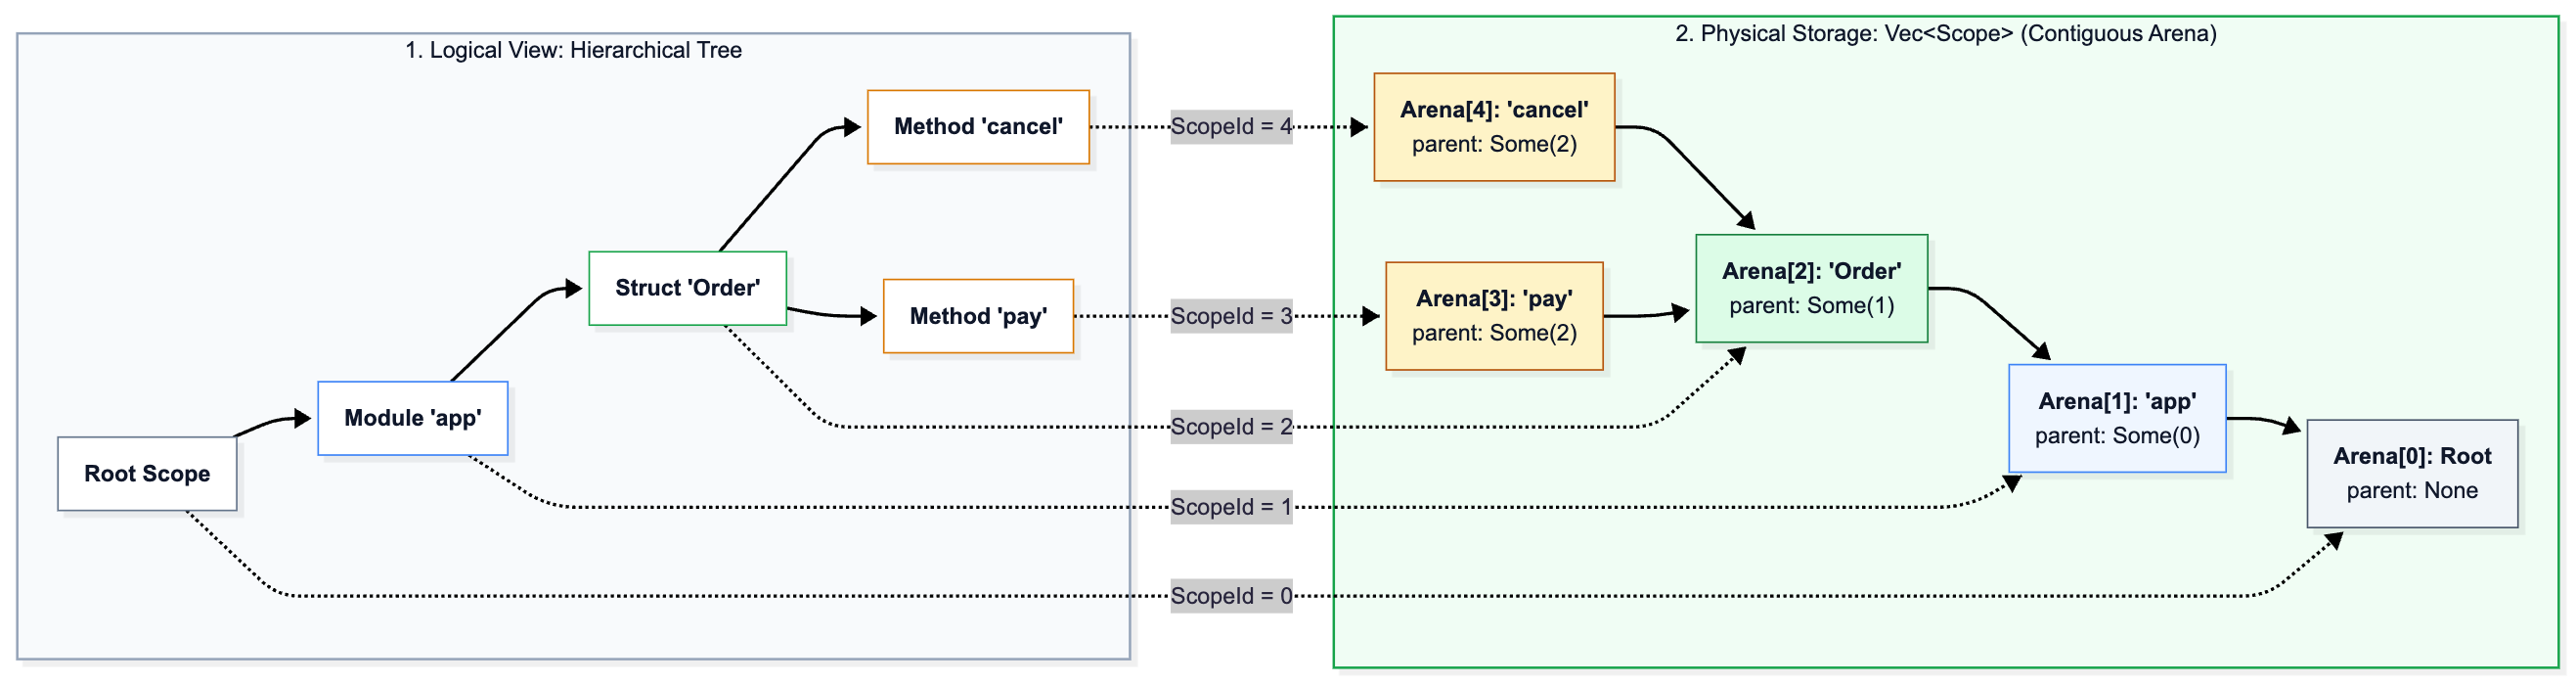
\includegraphics[width=\linewidth,height=0.52\textheight,keepaspectratio]{../images/name_resolution/scope_tree_arena.png}
      \vspace{0.2em}
      \captionof{figure}{\scriptsize Scope Tree Arena e risoluzione inter-procedurale.}
  \end{columns}

\end{frame}

% ==============================================================================
% SLIDE 12: FASE 3 - GRAPH CONSTRUCTION
% ==============================================================================
\begin{frame}{Fase 3: Costruzione e Proiezione del Grafo}
  \cookiekicker{DALL'ALBERO AL MULTIGRAFO}
  \vspace{0.1em}
  \begin{columns}[c,onlytextwidth]
    \column{0.48\textwidth}
      \begin{cookiecard}[title={Flattening ed Emissione Archi}]
        \small
        \begin{itemize}\setlength{\itemsep}{0.2em}
          \item \textbf{Node Flattening:} Denominazione univoca globale con \textbf{Qualified Names} ($\pi$) per tutti i vertici.
          \item \textbf{Archi Strutturali:} Contenimento (\texttt{belongsTo}) ed ereditarietà (\texttt{extends}, \texttt{implements}).
          \item \textbf{Archi Comportamentali:} Invocazioni (\texttt{calls}) e istanziazioni (\texttt{instantiates}).
          \item \textbf{Chiusura Referenziale:} Sintesi di vertici per librerie esterne e deduplicazione archi.
        \end{itemize}
      \end{cookiecard}

    \column{0.50\textwidth}
      \centering
      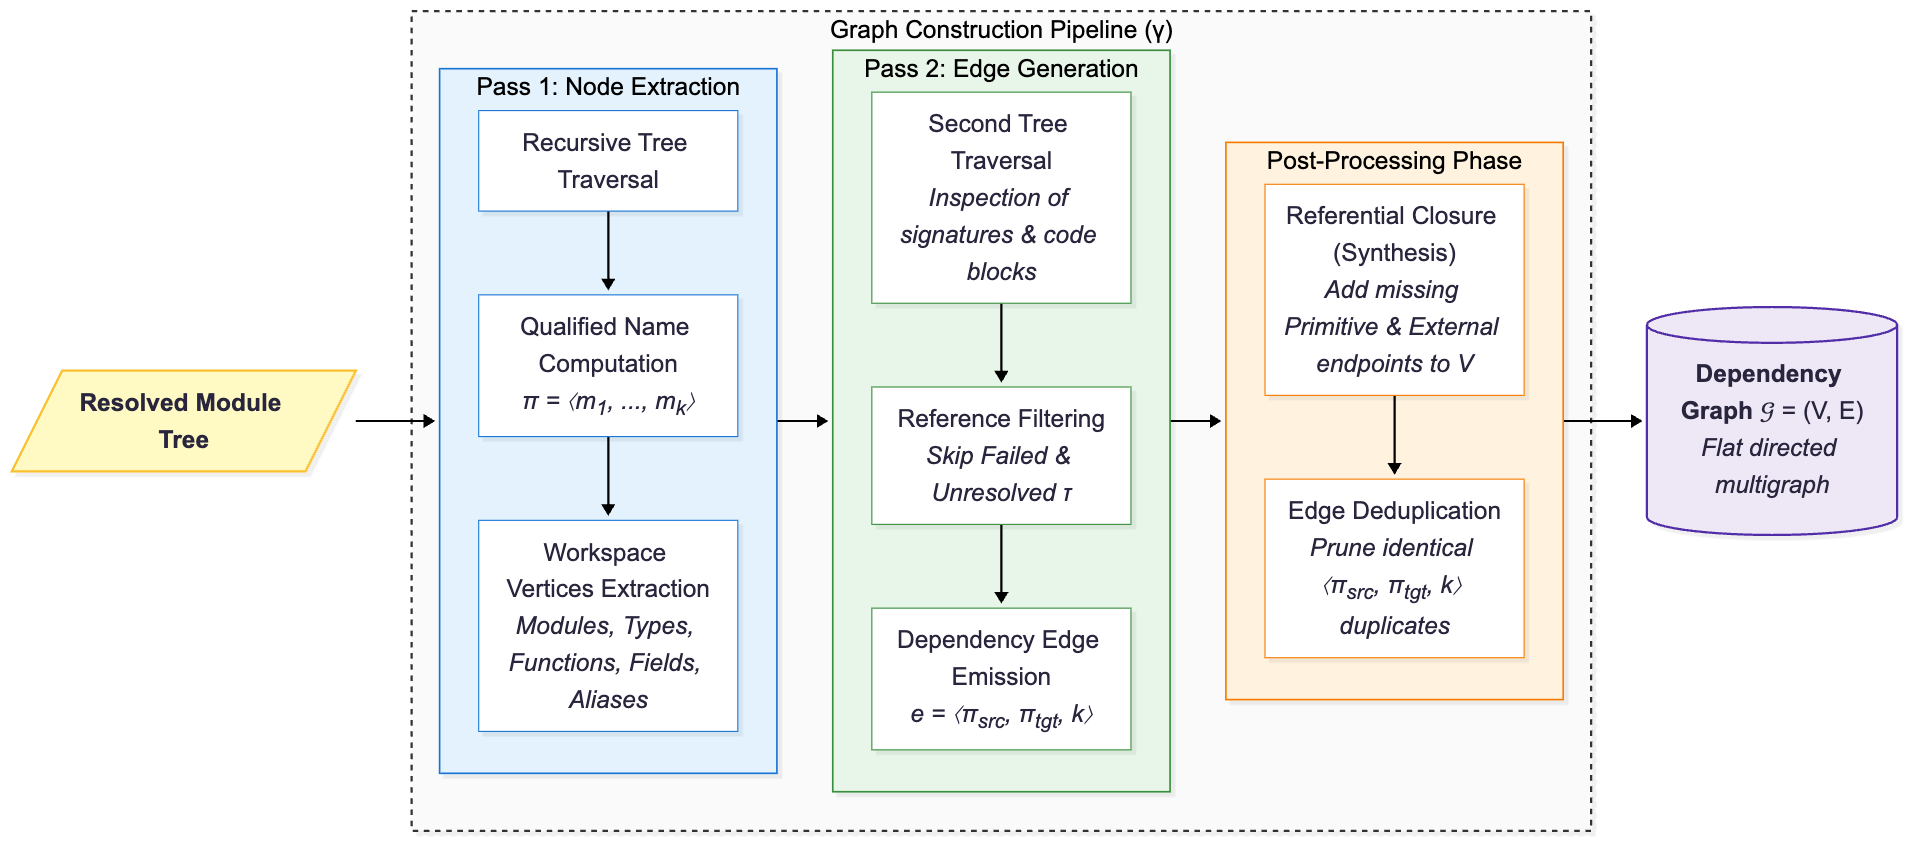
\includegraphics[width=\linewidth,height=0.52\textheight,keepaspectratio]{../images/graph_construction/graph_construction_pipeline.png}
      \vspace{0.2em}
      \captionof{figure}{\scriptsize Pipeline di generazione del grafo e deduplicazione archi.}
  \end{columns}

\end{frame}

% ==============================================================================
% SLIDE 13: METODOLOGIA DI VALUTAZIONE & RQS
% ==============================================================================
\begin{frame}{Metodologia di Validazione Sperimentale}
  \cookiekicker{FRAMEWORK SPERIMENTALE}
  \vspace{0.1em}
  \begin{columns}[c,onlytextwidth]
    \column{0.52\textwidth}
      \begin{cookiecard}[title={Le 4 Research Questions}]
        \small
        \begin{itemize}\setlength{\itemsep}{0.18em}
          \item \textbf{RQ1 (Construct Coverage):} Copertura costrutti linguistici su benchmark sintetici controllati.
          \item \textbf{RQ2 (Cross-Tool Alignment):} Allineamento strutturale dei grafi rispetto a tool consolidati su software reale.
          \item \textbf{RQ3 (Discrepancy Analysis):} Decomposizione divergenze per tipologia di dipendenza.
          \item \textbf{RQ4 (Scalability):} Throughput e scalabilità computazionale al crescere della dimensione.
        \end{itemize}
      \end{cookiecard}

    \column{0.45\textwidth}
      \begin{cookiecard}[title={Dataset \& Baselines}]
        \small
        \begin{itemize}\setlength{\itemsep}{0.2em}
          \item \textbf{156 Repository Open-Source} reali.
          \item Quasi \textbf{98 Milioni di LOC} analizzate.
          \item \textbf{5 Linguaggi:} Java, C, C++, Python, Rust.
          \item \textbf{Baselines di Confronto:}
            \begin{itemize}\setlength{\itemsep}{0.1em}
              \item \textbf{Arcan} (Bicocca)
              \item \textbf{Depends} (Multilinguaggio)
              \item \textbf{Entangle}
            \end{itemize}
        \end{itemize}
      \end{cookiecard}
  \end{columns}

\end{frame}

% ==============================================================================
% SLIDE 14: GRAPH HARMONIZATION FRAMEWORK
% ==============================================================================
\begin{frame}{Graph Harmonization: Benchmark Controllati}
  \cookiekicker{METODOLOGIA DI CONFRONTO EQUO}
  \vspace{0.1em}
  \begin{columns}[c,onlytextwidth]
    \column{0.50\textwidth}
      \begin{cookiecard}[title={I 4 Pilastri di Graph-Synchron}]
        \small
        \begin{enumerate}\setlength{\itemsep}{0.2em}
          \item \textbf{Canonical Path Normalization:} Percorsi unificati.
          \item \textbf{Semantic Entity Lifting:} Sollevamento membri ai tipi racchiudenti.
          \item \textbf{Package Synthesis:} Package intermedi mancanti.
          \item \textbf{Unified Taxonomy:} Mappatura semantica archi (\texttt{belongsTo}, \texttt{dependsOn}).
        \end{enumerate}
      \end{cookiecard}

    \column{0.48\textwidth}
      \begin{cookiecard}[title={Metrica di Similarità \& RQ1}]
        \small \textbf{Smoothed Jaccard Index:}
        $$J(A, B) = \frac{|A \cap B|}{|A \cup B|}$$
        Valutato su nodi ($J_{\text{nodes}}$) e archi ($J_{\text{edges}}$).
        \vspace{0.3em}\par
        \textbf{Risultato RQ1 (Micro-benchmarks):}\\
        \textbf{\color{metricGreen}100\% di oracoli superati} con conformità totale su tutti i 5 linguaggi.
      \end{cookiecard}
  \end{columns}

\end{frame}

% ==============================================================================
% SLIDE 15: RISULTATI RQ2 - ALLINEAMENTO JAVA & PYTHON
% ==============================================================================
\begin{frame}{Risultati RQ2: Allineamento su Larga Scala}
  \cookiekicker{VALIDAZIONE EMPIRICA SU 156 REPOSITORY}
  \vspace{0.1em}
  \begin{columns}[c,onlytextwidth]
    \column{0.48\textwidth}
      \begin{cookiecard}[title={Affidabilità ed Allineamento in Java}]
        \footnotesize
        \begin{itemize}\setlength{\itemsep}{0.18em}
          \item \textbf{Completion Rate:} OmniDeps \textbf{\color{metricGreen}99.4\%} (155/156) vs Depends (92.7\%), Arcan (49.2\%), Entangle (29.7\%).
          \item \textbf{Jaccard Java:} Nodi $0.814$ (Depends), $0.770$ (Entangle); Archi $\approx 0.59$.
          \item \textbf{Omissione Minima:} Omette solo lo \textbf{0.3\%} di nodi vs Arcan e il \textbf{2.1\%} vs Depends.
          \item \textbf{Python \& Rust:} Jaccard nodi 0.740 su Python; 32/32 progetti estratti con successo su Rust.
        \end{itemize}
      \end{cookiecard}

    \column{0.50\textwidth}
      \centering
      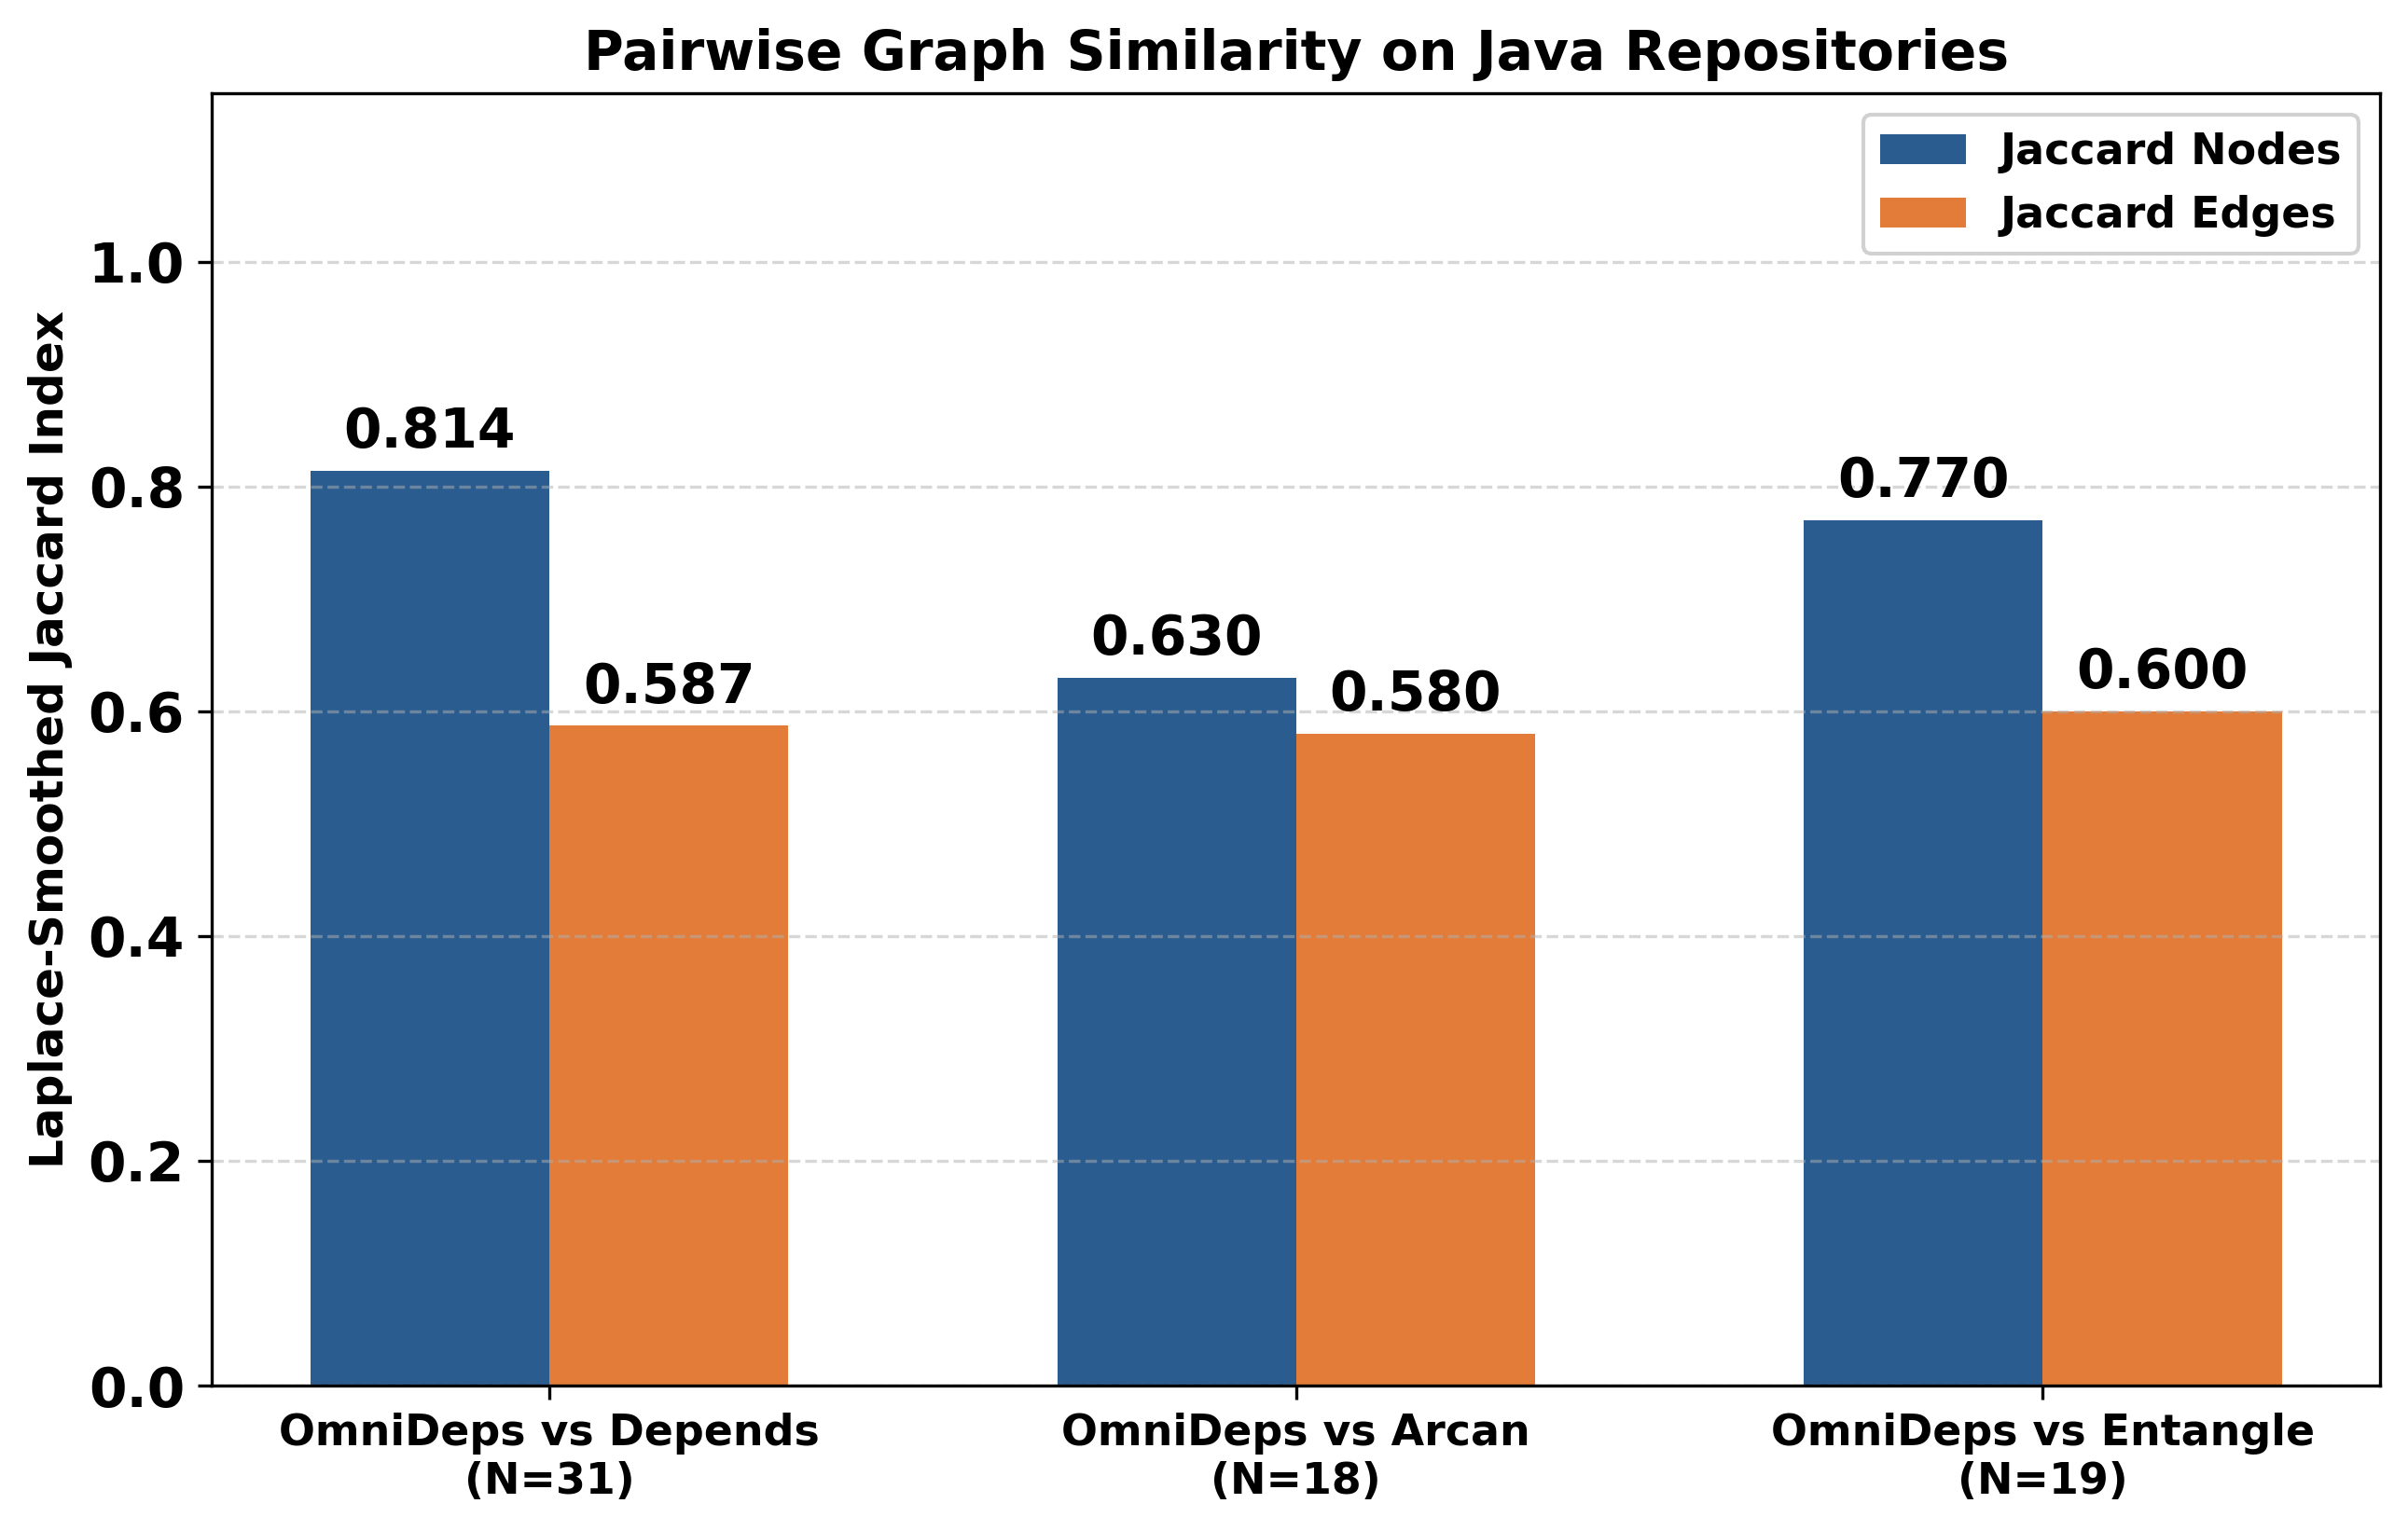
\includegraphics[width=\linewidth,height=0.52\textheight,keepaspectratio]{../images/evaluation/comparisons/summary-jaccard-java.png}
      \vspace{0.2em}
      \captionof{figure}{\scriptsize Indici di Jaccard su nodi ed archi per Java rispetto alle baseline.}
  \end{columns}

\end{frame}

% ==============================================================================
% SLIDE 16: RISULTATI RQ3 - IL CASO C/C++ E PREPROCESSING
% ==============================================================================
\begin{frame}{Risultati RQ3: Il Caso C/C++ e Preprocessing}
  \cookiekicker{ANALISI DELLE DISCREPANZE}
  \vspace{0.1em}
  \begin{columns}[c,onlytextwidth]
    \column{0.50\textwidth}
      \begin{cookiecard}[title={Discrepanze in C e C++}]
        \small
        \begin{itemize}\setlength{\itemsep}{0.2em}
          \item \textbf{Arcan (Divergenza Ontologica):} Arcan modella file e header (\texttt{.c}/\texttt{.h}); OmniDeps modella i tipi (\texttt{struct}/\texttt{class}). Vertici disgiunti per design.
          \item \textbf{Depends (Effetto Preprocessing):}
            \begin{itemize}\setlength{\itemsep}{0.1em}
              \item L'espansione macro raddoppia la similarità archi ($0.081 \rightarrow 0.165$).
              \item L'inlining degli header standard gonfia il denominatore Jaccard.
            \end{itemize}
          \item \textbf{Codebase Modulari:} Accordo totale su \texttt{sds} ($J = 1.0$), forte su \texttt{ninja} ($0.41$) e \texttt{re2} ($0.46$).
        \end{itemize}
      \end{cookiecard}

    \column{0.48\textwidth}
      \centering
      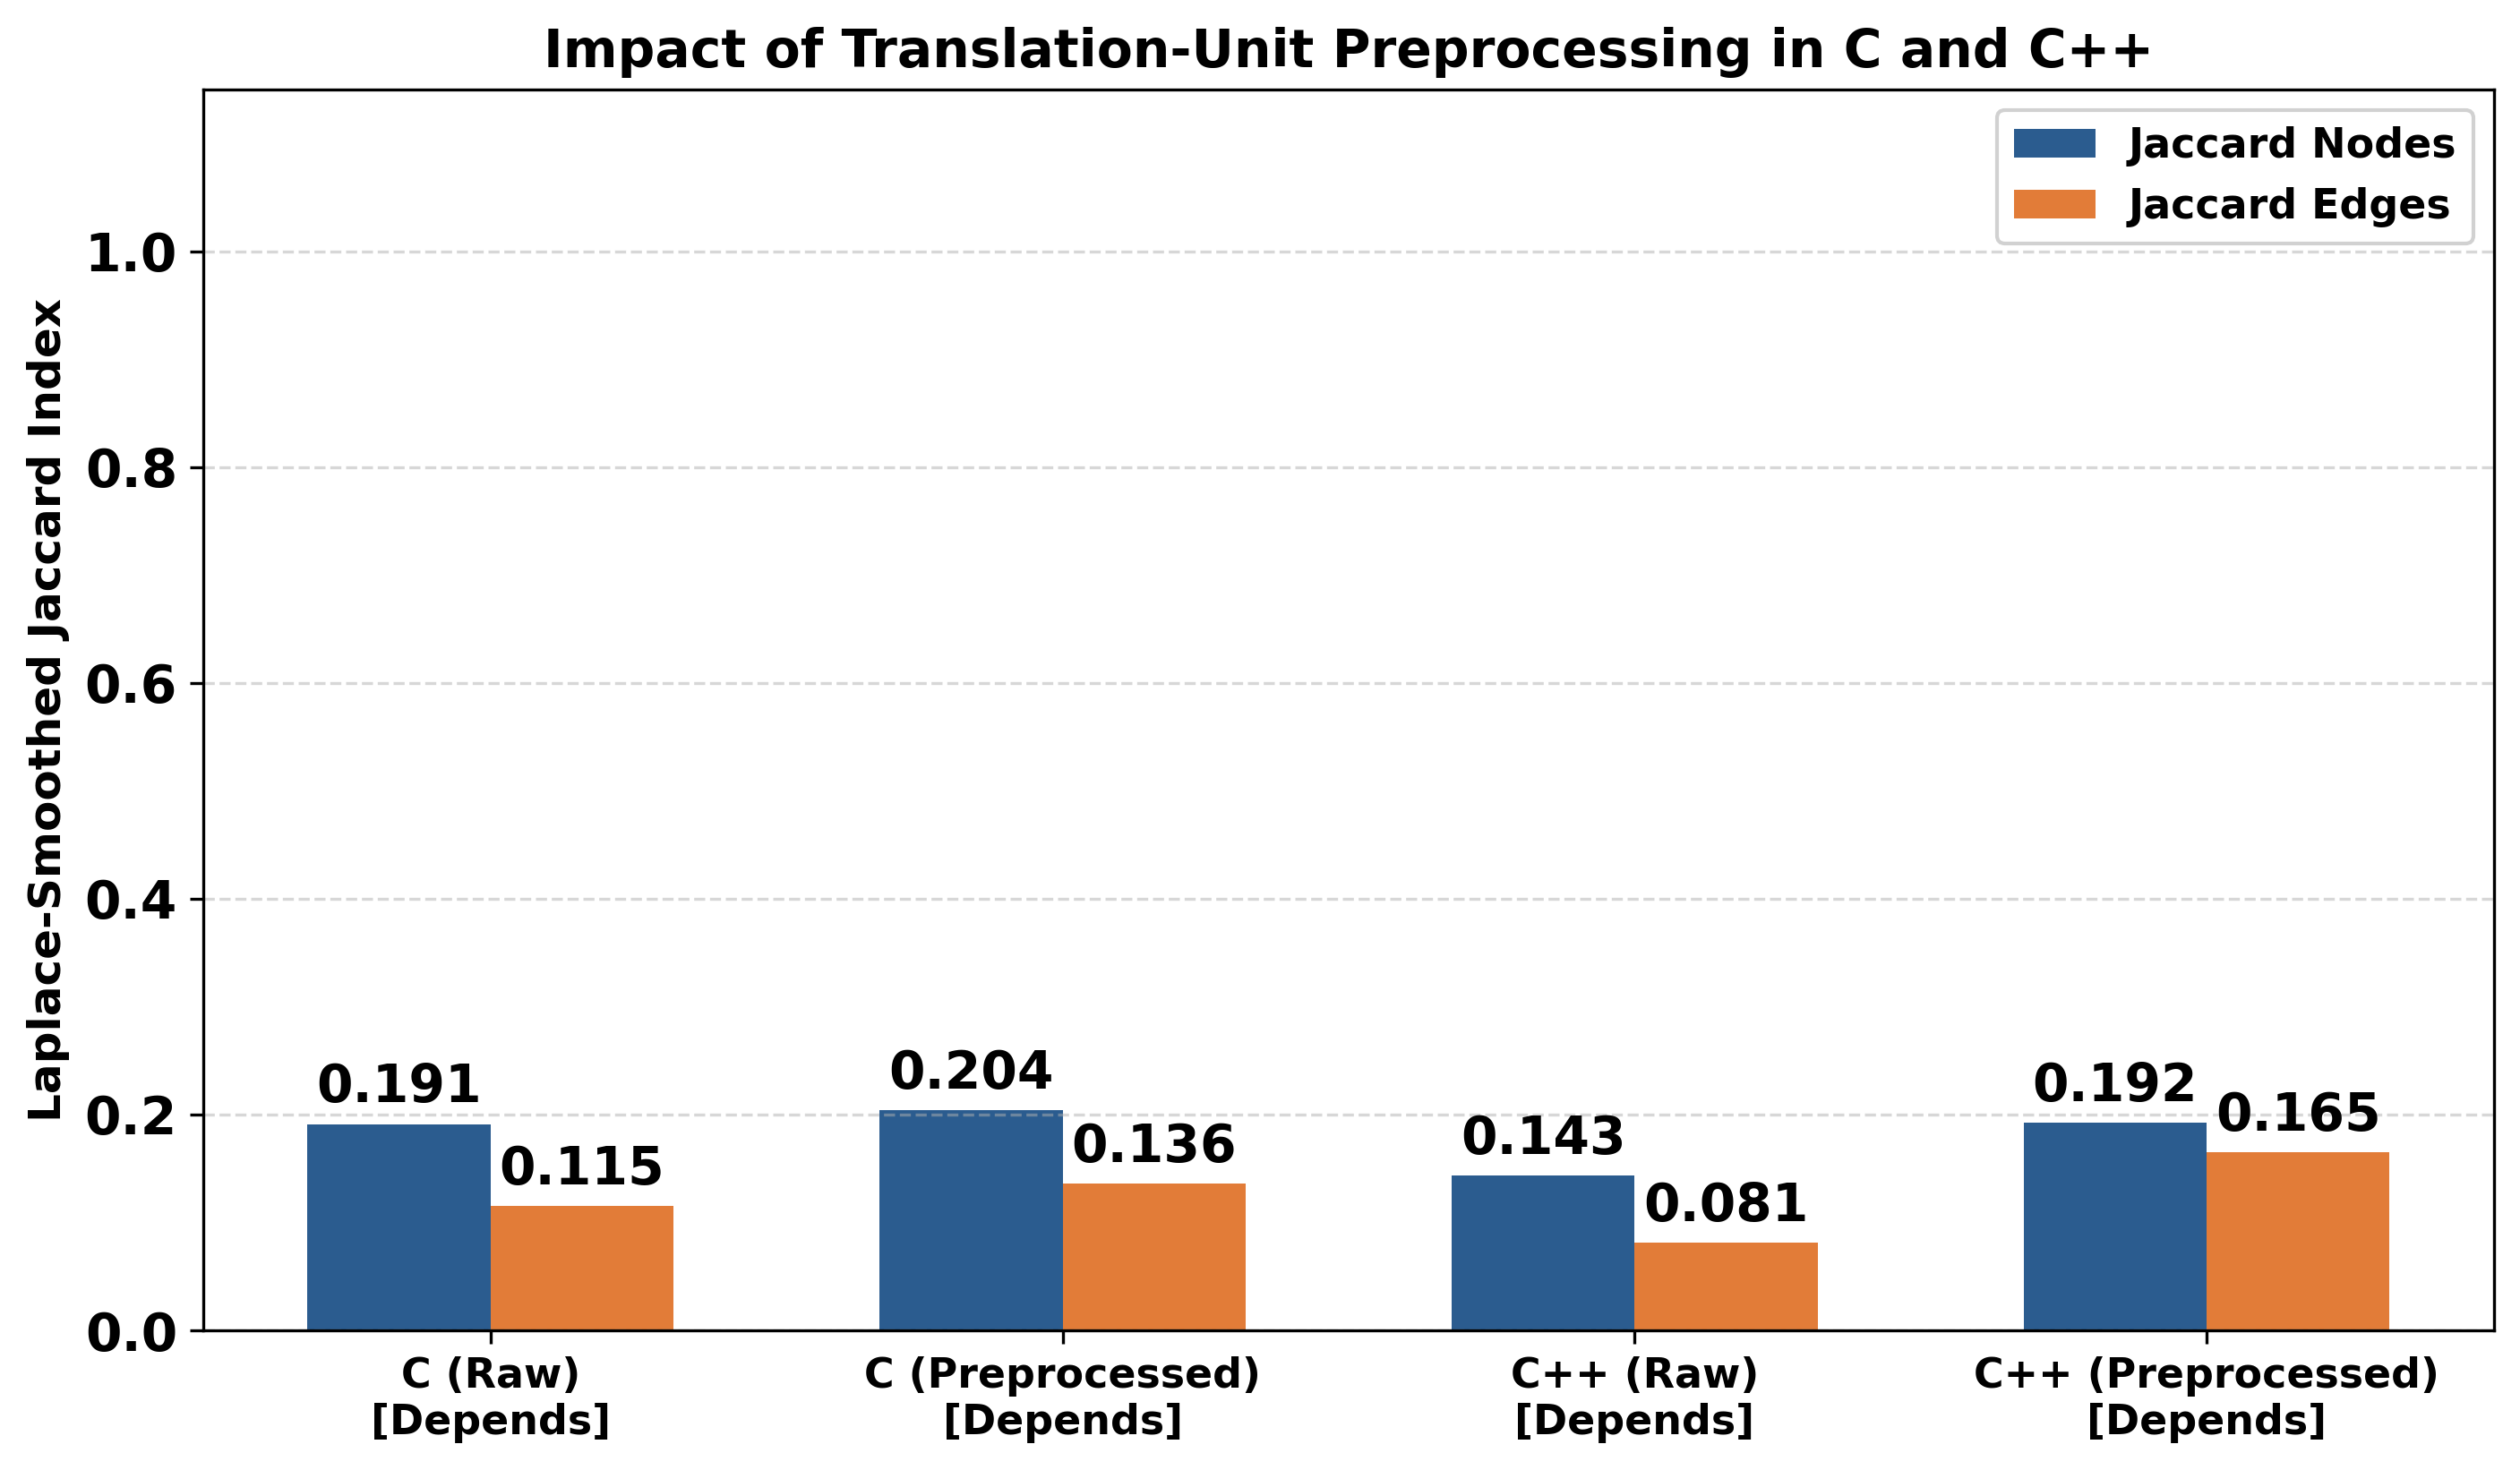
\includegraphics[width=\linewidth,height=0.52\textheight,keepaspectratio]{../images/evaluation/comparisons/summary-jaccard-c-cpp-preprocessing.png}
      \vspace{0.2em}
      \captionof{figure}{\scriptsize Impatto del preprocessing su C e C++.}
  \end{columns}

\end{frame}

% ==============================================================================
% SLIDE 17: RISULTATI RQ4 - PRESTAZIONI & SCALABILITÀ
% ==============================================================================
\begin{frame}{Risultati RQ4: Prestazioni e Scalabilità}
  \cookiekicker{THROUGHPUT E SCALABILITÀ COMPUTAZIONALE}
  \vspace{0.1em}
  \begin{columns}[c,onlytextwidth]
    \column{0.48\textwidth}
      \begin{cookiecard}[title={Throughput \& Speedup di OmniDeps}]
        \small
        \begin{itemize}\setlength{\itemsep}{0.2em}
          \item \textbf{Throughput Medio:} \textbf{\color{metricGreen} 74.445 LOC/s} (picchi oltre \textbf{97.000 LOC/s} su Rust).
          \item \textbf{Speedup vs Depends:} \textbf{13.2x} in media (fino a 74x su Python e 79x su C).
          \item \textbf{Speedup vs Arcan:} \textbf{48.2x} in media (fino a 116x su Java e 536x su C).
          \item \textbf{Speedup vs Entangle:} \textbf{4.0x} in media.
          \item \textbf{Complessità Lineare:} Scalabilità $O(N)$, ideale per pipeline di Continuous Integration (CI/CD).
        \end{itemize}
      \end{cookiecard}

    \column{0.50\textwidth}
      \centering
      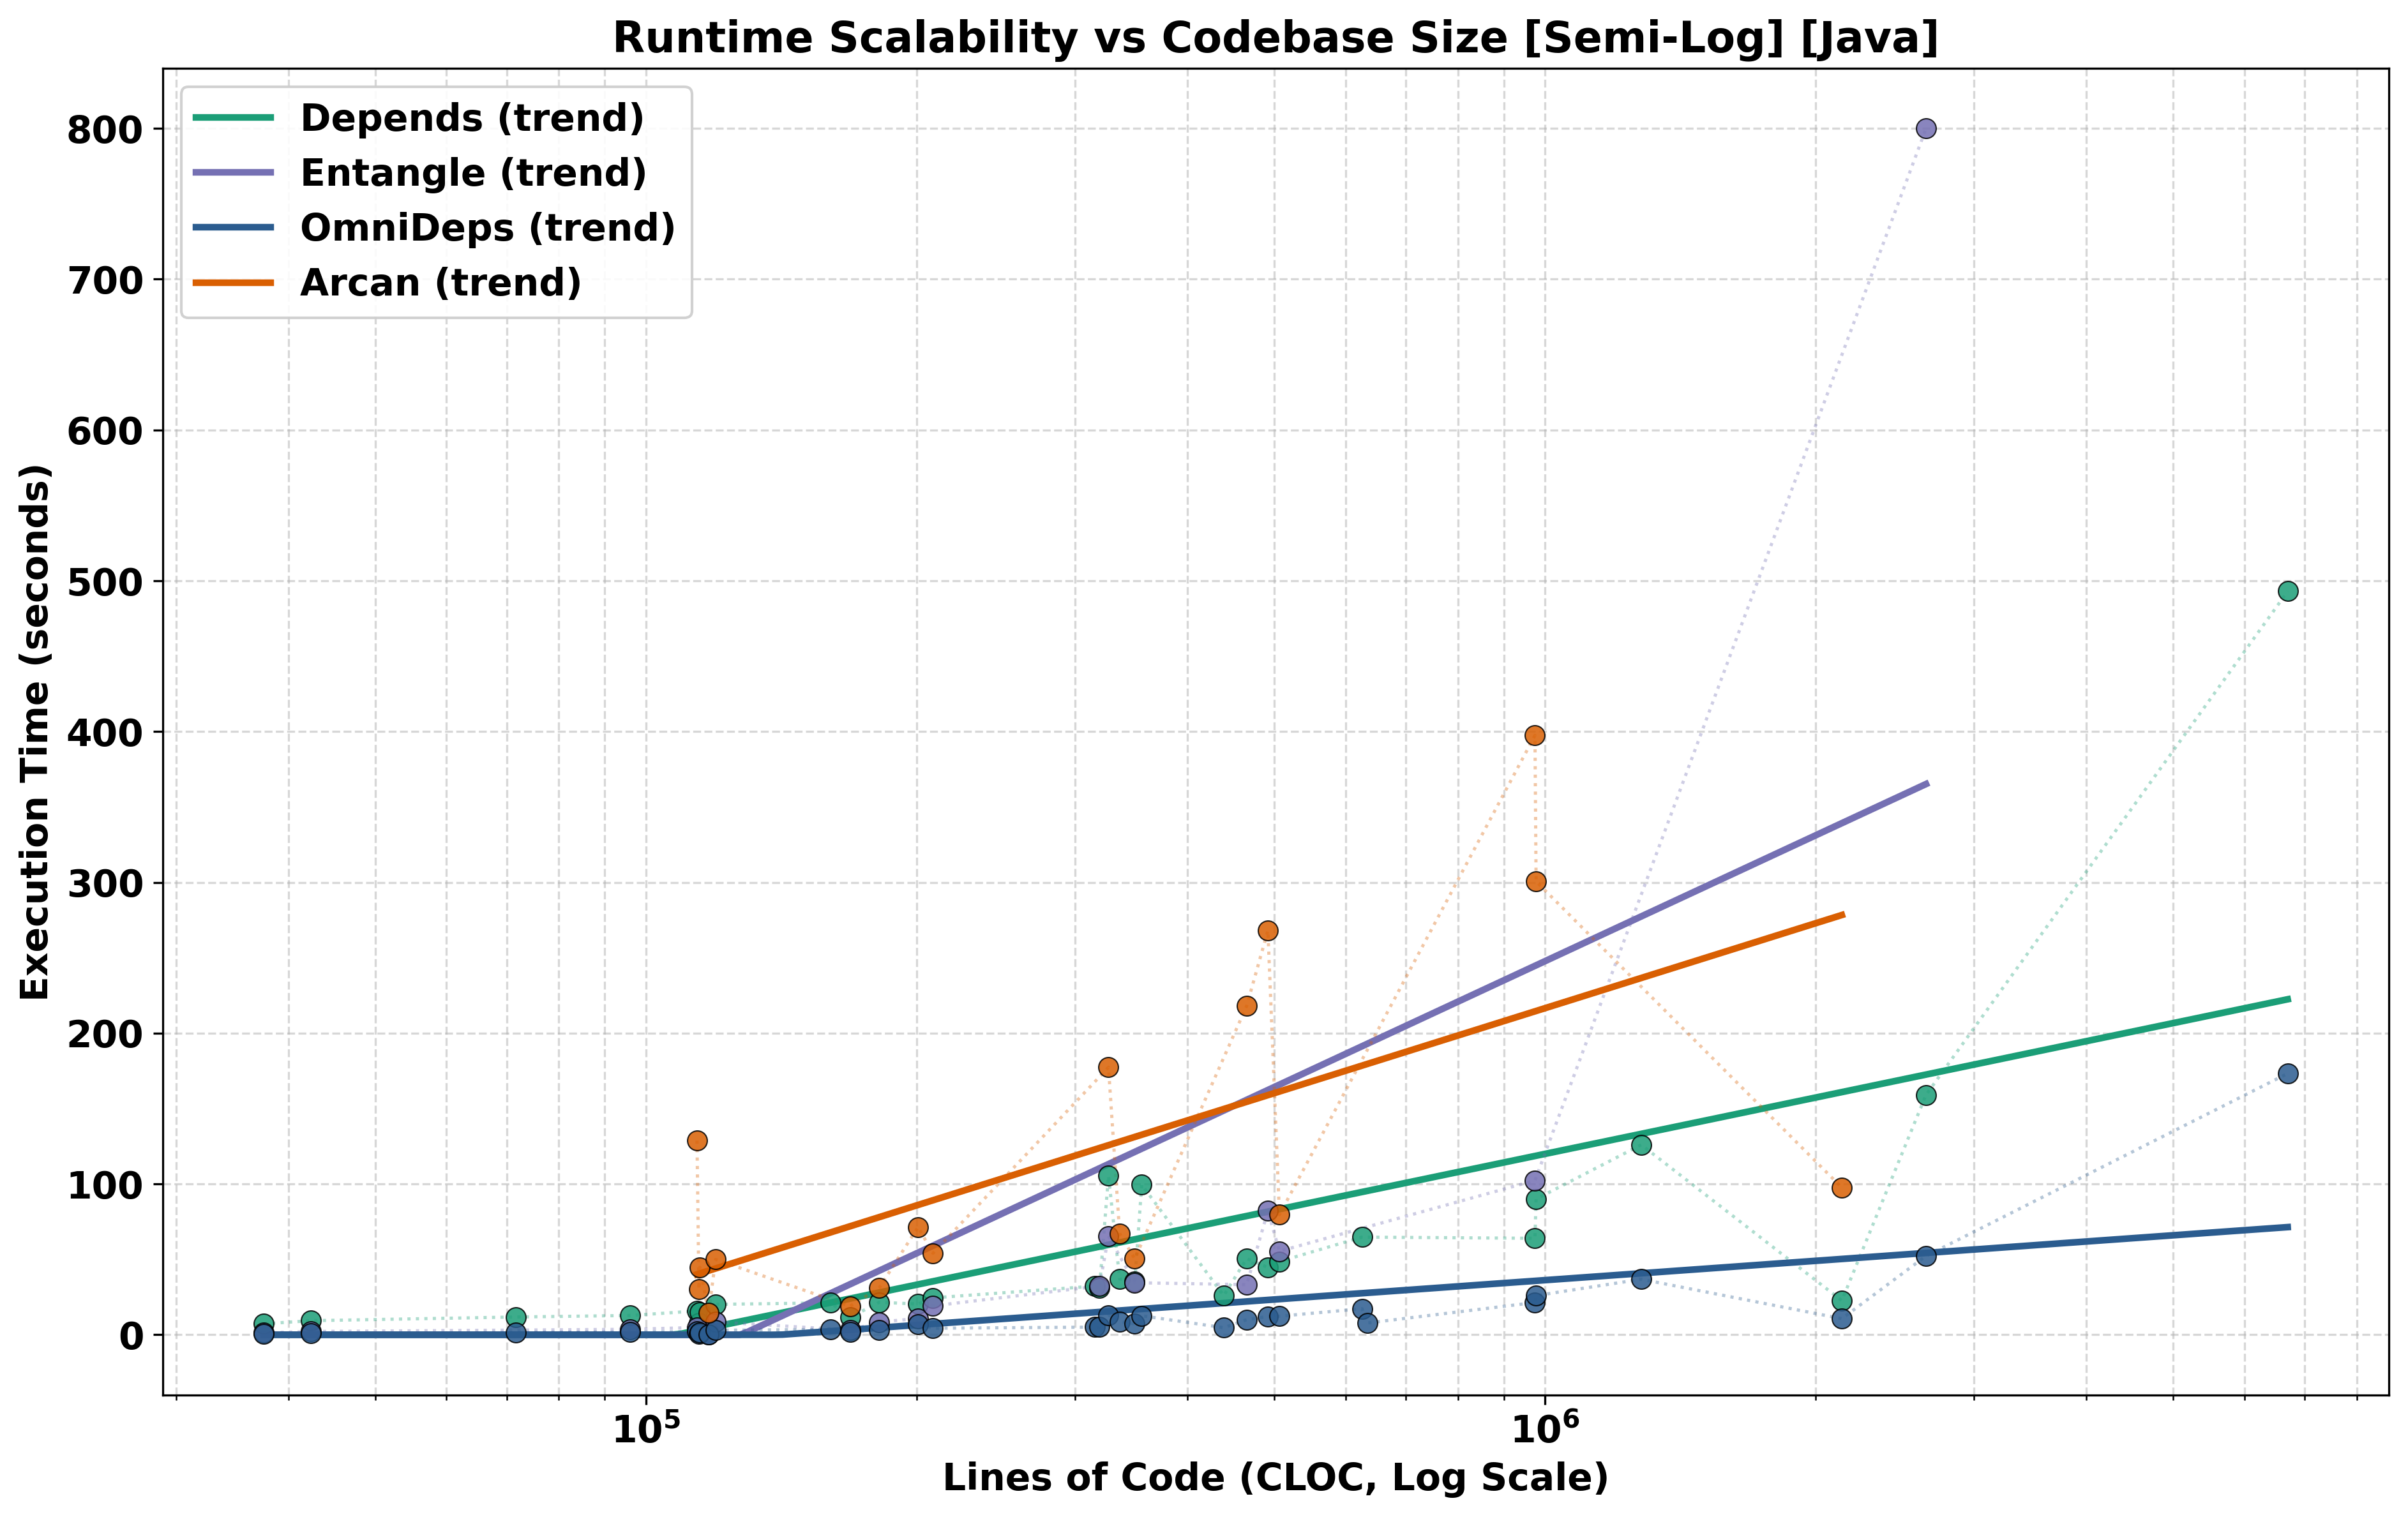
\includegraphics[width=\linewidth,height=0.52\textheight,keepaspectratio]{../images/evaluation/times/graph-cloc-log-java.png}
      \vspace{0.2em}
      \captionof{figure}{\scriptsize Scalabilità semi-logaritmica tempo vs LOC in Java.}
  \end{columns}

\end{frame}

% ==============================================================================
% SLIDE 18: DISCUSSIONE DEI TRADE-OFF
% ==============================================================================
\begin{frame}{Discussione: Trade-off Architetturali}
  \cookiekicker{RIFLESSIONE CRITICA}
  \vspace{0.1em}
  \begin{columns}[c,onlytextwidth]
    \column{0.49\textwidth}
      \begin{cookiecard}[title={Punti di Forza Dimostrati}]
        \small
        \begin{itemize}\setlength{\itemsep}{0.2em}
          \item \textbf{Zero Build Configuration:} Nessuna configurazione di SDK o compiler nativi.
          \item \textbf{Singola Architettura:} Estendibile a nuovi linguaggi con sole euristiche di Fase 1.
          \item \textbf{Throughput Estremo:} Memoria controllata e analisi di grandi progetti in secondi.
        \end{itemize}
      \end{cookiecard}

    \column{0.49\textwidth}
      \begin{cookiecard}[title={Compromessi Riconosciuti}]
        \small
        \begin{itemize}\setlength{\itemsep}{0.2em}
          \item \textbf{Binari Esterni:} Catene che attraversano librerie chiuse non propagano il tipo.
          \item \textbf{Linguaggi Dinamici:} In Python, accuratezza legata alla presenza di Type Hint.
          \item \textbf{Preprocessore C/C++:} Trade-off tra espansione macro e rumore da header.
        \end{itemize}
      \end{cookiecard}
  \end{columns}
  \vspace{0.4em}
  \centering
  {\small\textbf{Trade-off Fondamentale:} \textit{Compiler Precision} $\longleftrightarrow$ \textit{Lightweight Scalability per CI/CD}}

\end{frame}

% ==============================================================================
% SLIDE 19: CONCLUSIONI E SVILUPPI FUTURI
% ==============================================================================
\begin{frame}{Conclusioni e Sviluppi Futuri}
  \cookiekicker{TRAGUARDI E VISIONE}
  \vspace{0.1em}
  \begin{columns}[c,onlytextwidth]
    \column{0.48\textwidth}
      \begin{cookiecard}[title={Contributi Principali}]
        \small
        \begin{itemize}\setlength{\itemsep}{0.2em}
          \item \textbf{Teoria:} IR universale formale basata su ADT e risoluzione dei nomi via Query Algebra.
          \item \textbf{Ingegneria:} Framework \textbf{OmniDeps} in Rust ad alte prestazioni (74k+ LOC/s).
          \item \textbf{Validazione:} Graph Harmonization e benchmark su 156 repository ($\sim$98M LOC).
        \end{itemize}
      \end{cookiecard}

    \column{0.48\textwidth}
      \begin{cookiecard}[title={Direzioni Future}]
        \small
        \begin{itemize}\setlength{\itemsep}{0.2em}
          \item \textbf{Parallelizzazione Multi-threading:} Estrazione concorrente dei file tramite Rayon.
          \item \textbf{Analisi Cross-Language:} Tracciamento inter-linguaggio (JNI Java-C/C++, FFI Rust/Python/C).
          \item \textbf{Estensione di Paradigma:} Supporto a linguaggi funzionali o dichiarativi.
        \end{itemize}
      \end{cookiecard}
  \end{columns}
  \vspace{0.4em}
  \centering
  \cookiebadge{Language-Agnostic} \quad \cookiebadge{High-Throughput} \quad \cookiebadge{Open Science}

\end{frame}

% ==============================================================================
% SLIDE 20: CHIUSURA & Q&A
% Slide personalizzata con sfondo Unimib Blue, QR code Zenodo e niente mascotte
% ==============================================================================
\begin{frame}[plain,noframenumbering]
  
\begin{tikzpicture}[remember picture,overlay]
    \fill[unimibBlue] (current page.south west) rectangle (current page.north east);
    % Cerchi decorativi
    \draw[white,opacity=0.08,line width=3pt] ($(current page.north east)+(-0.15\paperwidth,-0.15\paperheight)$) circle[radius=0.18\paperheight];
    \draw[white,opacity=0.05,line width=2pt] ($(current page.south west)+(0.20\paperwidth,0.20\paperheight)$) circle[radius=0.12\paperheight];
  \end{tikzpicture}%
  \vspace*{0.02\paperheight}%
  \begin{columns}[c,onlytextwidth]
    \column{0.60\textwidth}
      {\usebeamerfont{cookie kicker}\color{white!75} CONCLUSIONS \& Q\&A}\par\vspace{0.4em}
      {\fontsize{21}{25}\selectfont\bfseries\color{white} Thank you for your attention!}\par\vspace{0.6em}
      {\small\color{white!90}\textbf{A Language-Agnostic Framework\\ for Dependency Extraction}}\par\vspace{0.6em}
      {\color{white!40}\rule{0.25\paperwidth}{1pt}}\par\vspace{0.8em}
      {\footnotesize\color{white!90}\textbf{Candidate:} Christian Ferrario}\quad{\scriptsize\color{white!75}(\url{c.ferrario30@campus.unimib.it})}\par\vspace{0.4em}
      {\footnotesize\color{white!90}\textbf{Supervisor:} Prof. Francesca Arcelli Fontana\par}
      {\footnotesize\color{white!90}\textbf{Co-Supervisor:} Dr. Francesco Refolli\par}
      \vspace{1.1em}
      {\small\itshape\color{white!80} Open for questions and discussion}

    \column{0.36\textwidth}
      \centering
      \begin{tcolorbox}[
        colback=white,
        colframe=white,
        arc=3mm,
        boxrule=0pt,
        width=0.88\linewidth,
        halign=center,
        valign=center,
        top=4mm,bottom=4mm,left=3mm,right=3mm
      ]
        \href{https://doi.org/10.5281/zenodo.23315197}{\color{black}\qrcode[height=2.3cm]{https://doi.org/10.5281/zenodo.23315197}}
        \vspace{0.4em}\par
        {\footnotesize\bfseries\color{unimibBlue} Zenodo Artifact}\par
        {\tiny\color{cookieMuted} DOI: 10.5281/zenodo.23315197\par}
        {\tiny\color{cookieMuted} Dataset, Benchmark \& Source Code}
      \end{tcolorbox}
  \end{columns}

\end{frame}

\end{document}
